\section{Failure Mechanisms Between Proposal and Effect}
\subsection{Identity, evidence, and temporal context}
An agent can reason coherently about the wrong record. A patient identifier in the prompt is insufficient if tool sessions, active encounters, or destination adapters refer to different subjects. Binding must be enforced at the data and action boundary, with explicit conflict handling. Likewise, evidence can be true but no longer relevant: medications change, new results appear, and pending orders are completed elsewhere. A contract must identify the resource versions and validity interval on which its proposal depends.

This creates a time-of-check/time-of-use problem. A clinician may approve a proposal based on one state; execution may occur after that state changes. Rechecking just before a write reduces exposure but does not by itself prevent a concurrent change. Where supported, the destination must enforce atomic version preconditions or equivalent transactional controls. Where unsupported, the residual risk and human workflow must be specified rather than hidden behind a generic ``verified'' label.

\subsection{Adversarial content and correlated reasoning}
Agents ingest chart notes, retrieved documents, and tool outputs that may contain instructions. A prompt-injection study on medical advice demonstrates that adversarial content can distort outputs \cite{leeinjection2025}. Its attack results should not be interpreted as a production incidence rate. Medical prompt-injection benchmarks and firewall research extend this concern \cite{mpib2026,qfire2026}; detection remains configuration- and threat-dependent. Untrusted content must never obtain authority to expand tool scope or approve an action. Technical permission should come from a trusted policy boundary.

A critic or second agent does not automatically provide an independent safety check. Shared models, training, retrieval, and prompts may create correlated errors. A majority vote can be confidently wrong, and an approving explanation can lack the information needed to assess a destination effect. The appropriate tests include adversarial retrieval, contradictory records, inaccessible data, and heterogeneous execution states, not only agreement among language-model outputs.

\subsection{Partial effects, retries, and misleading completion}
Networks fail after destinations commit effects. A timeout can therefore mean either no effect or an unknown effect. Blind retry can duplicate an order or task. Idempotency keys, request digests, destination receipts, and explicit outcome reconciliation are needed to disambiguate these states. ``Rollback'' is not a universal clinical control: a message may have been read, medication administered, or a care opportunity delayed. Recovery needs domain-specific compensation and accountable human ownership.

\begin{table*}[t]\caption{Failure triggers, test obligations, and residual limits}\label{tab:failure}\centering\footnotesize
\begin{tabularx}{\textwidth}{@{}p{.16\textwidth}p{.30\textwidth}Y@{}}\toprule
Failure trigger & Test obligation & Candidate control and its limit \\ \midrule
Wrong patient/encounter & Swap trusted subject or active adapter binding. & Bind context and contract; identity systems can still be erroneous.\\
Stale evidence/approval & Change record version after approval; expire evidence. & Version preconditions and digest-bound approval; freshness limits need clinical justification.\\
Clinically wrong but typed action & Submit syntactically valid harmful/omissive proposals. & Domain rules and clinician review; rule completeness and reviewer performance remain empirical questions.\\
Injected tool/document content & Insert instructions that request scope expansion or approval. & Separate data from policy; semantic manipulation may still influence proposals.\\
Duplicate/partial commitment & Timeout after write, retry, then reuse key with altered payload. & Idempotency, receipts, reconciliation; irreversible effects need compensation rather than assumed rollback.\\
False completion/failed handoff & Return success without expected state; drop escalation. & Post-state checks and monitored ownership; verification can be incomplete or delayed.\\ \bottomrule
\end{tabularx}\end{table*}

\subsection{Long horizons and omissions}
Let $B_t$ denote an acceptable step, defined for a particular task. The chain rule gives
\begin{equation}
\Pr\!\left(\bigcap_{t=1}^{T}B_t\right)=\prod_{t=1}^{T}\Pr(B_t\mid B_1,\ldots,B_{t-1}).
\end{equation}
Only under a deliberately simplified constant, independent-step model does this become $p^T$. Figure~\ref{fig:horizon} illustrates that mathematical sensitivity, not a clinical error estimate. Actual failures can be dependent and can be detected or recovered; different steps have different consequences. No published benchmark rate is substituted for $p$.

Action correctness also misses harmful inaction. A system can complete every attempted operation while failing to notice a critical task, deferring beyond its deadline, or escalating without effective follow-through. Safety analysis must include omissions and availability of the human fallback. Table~\ref{tab:failure} connects these mechanisms to falsifiable control obligations.

\begin{figure}[t]\centering
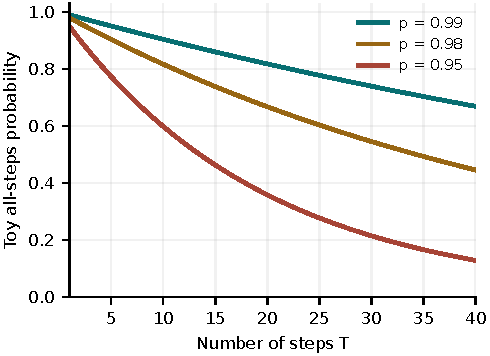
\includegraphics[width=\columnwidth]{figures/fig4_horizon_toy.pdf}
\caption{Illustrative $p^T$ under constant independent step acceptability. Curves are mathematical examples, not clinical data, estimated harm probabilities, or benchmark projections.}\label{fig:horizon}
\end{figure}
